\chapter{METODE PENELITIAN}\label{cha:metode}

\section{Waktu dan Tempat Pelaksanaan Penelitian}
Penelitian ini dilaksanakan pada bulan Februari 2024 di Jalan Desa Cipadung, Gang Bho Optikal, RT 03 RW 04, Kosan Armani Nomor 104, Cibiru, Kota Bandung, Jawa Barat 40614. Pemilihan waktu ini didasarkan pada ketersediaan peralatan dan kondisi lingkungan yang mendukung untuk pelaksanaan eksperimen.

Penelitian menggunakan alat yang dirancang khusus dengan tingkat presisi yang memadai untuk mengukur koefisien restitusi bola. Alat ini dilengkapi dengan sistem penyangga yang stabil untuk meminimalkan gangguan selama pengambilan data.

\begin{figure}
    \centering
    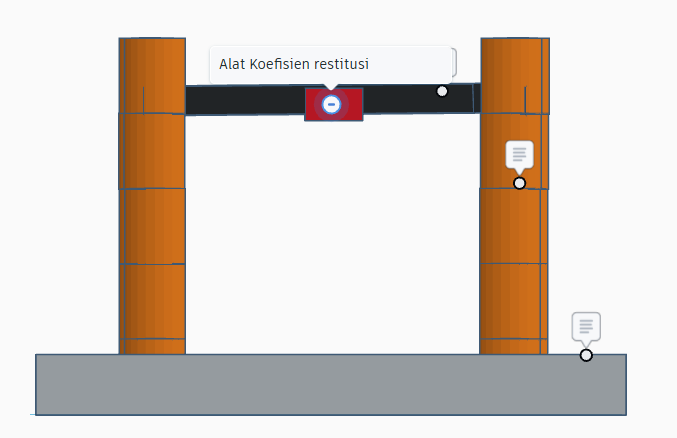
\includegraphics[width = 18pc]{images/Ilustrasi Alat.png}
    \caption{Ilustrasi Alat}
    \label{fig:ilustrasi_alat}
\end{figure}

Alat penelitian terdiri dari rangka penyangga dan wadah yang dirancang untuk menjaga stabilitas sensor selama proses pengukuran berlangsung.

\begin{figure}
    \centering
    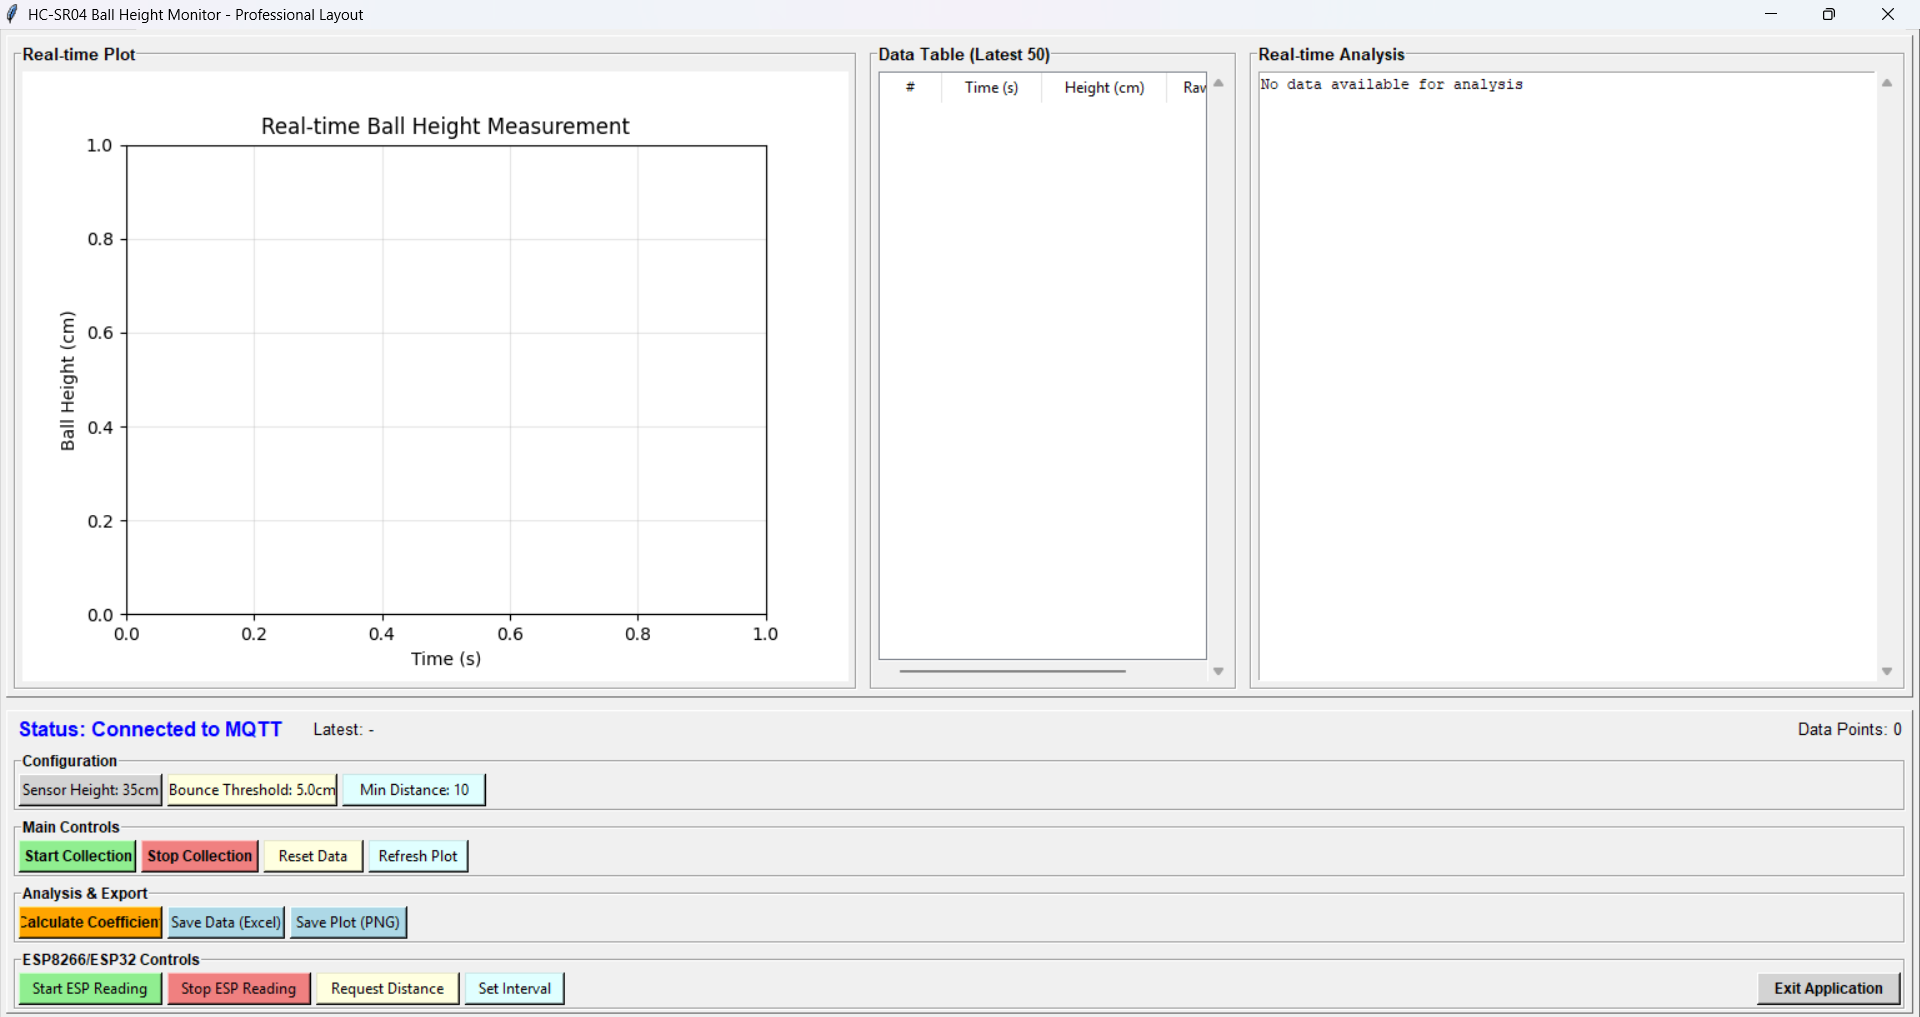
\includegraphics[width =\textwidth]{images/Tampilan GUI.png}
    \caption{Tampilan GUI}
    \label{fig:tampilan_gui}
\end{figure}

Aplikasi yang dikembangkan menggunakan bahasa pemrograman Python dengan antarmuka grafis berbasis Tkinter. Sistem ini memanfaatkan protokol MQTT untuk komunikasi jarak jauh antara sensor dan komputer. Data yang diperoleh dari sensor HC-SR04 dikirim melalui ESP8266 ke aplikasi untuk dianalisis secara real-time.

Antarmuka aplikasi terdiri dari panel kontrol untuk mengirim perintah, grafik untuk menampilkan data secara langsung, dan bagian analisis untuk menghitung koefisien restitusi. Komunikasi menggunakan broker MQTT HiveMQ dengan protokol QoS level 1 untuk memastikan data terkirim dengan baik.

\begin{figure}
    \centering
    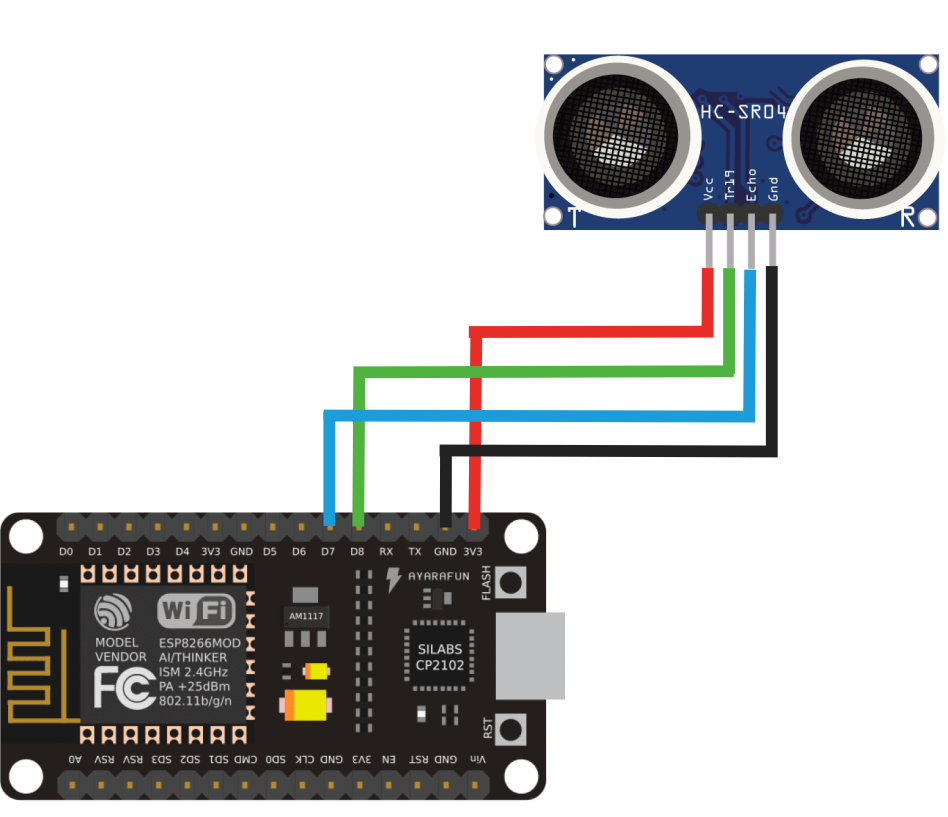
\includegraphics[width=0.5\linewidth]{images/Skematik Rangkaian.png}
    \caption{Skematik rangkaian}
    \label{fig:skematik_rangkaian}
\end{figure}

Rangkaian elektronik terdiri dari sensor HC-SR04 yang dihubungkan dengan mikrokontroler ESP8266. Pin VCC sensor dihubungkan ke pin 3V ESP8266, pin GND ke GND, pin TRIG ke pin D8, dan pin ECHO ke pin D7. Konfigurasi ini dapat disesuaikan dengan kebutuhan.

Pengujian dilakukan sebanyak 100 kali dengan menggunakan lima jenis bola yang berbeda. Setiap jenis bola diuji 20 kali untuk mendapatkan data yang cukup untuk analisis statistik.

\section{Alat dan Bahan Penelitian}

\subsection{Alat Penelitian}
Peralatan yang digunakan dalam penelitian ini tercantum dalam tabel berikut:

\begin{table}[H]
\caption{Daftar Peralatan Penelitian}
\label{tab:alat}
\begin{center}
    \begin{tabular}{|l|l|l|}
    \hline
        \textbf{No} & \textbf{Alat Penelitian} & \textbf{Jumlah} \\\hline
        1 & Laptop & 1 buah \\\hline
        2 & ESP8266 & 1 buah \\\hline
        3 & Sensor HC-SR04 & 1 buah \\\hline
        4 & Kabel jumper & Secukupnya \\\hline
        5 & Akrilik & Secukupnya \\\hline
        6 & Pipa besi & Secukupnya \\\hline
        7 & Mur dan baut & Secukupnya \\\hline
        8 & Penyambung pipa & Secukupnya \\\hline
        9 & Perangkat lunak Arduino IDE & - \\\hline
    \end{tabular}
\end{center}
\end{table}

\subsection{Bahan Penelitian}
Bahan-bahan yang digunakan sebagai objek pengujian adalah:

\begin{table}[H]
\caption{Daftar Bahan Penelitian}
\label{tab:bahan}
\begin{center}
    \begin{tabular}{|l|l|l|}
    \hline
        \textbf{No} & \textbf{Bahan Penelitian} & \textbf{Jumlah} \\\hline
        1 & Bola ping-pong & 1 buah \\\hline
        2 & Bola bekel & 1 buah \\\hline
        3 & Bola sepak karet & 1 buah \\\hline
        4 & Bola plastik & 1 buah \\\hline
        5 & Bola tenis lapangan & 1 buah \\\hline
    \end{tabular}
\end{center}
\end{table}

\section{Diagram Alir Penelitian}
\subsection{Diagram Alir Program Python}

\begin{figure}[H]
\centering
\begin{tikzpicture} [
    node distance=0.5cm,
    start/.style={ellipse, draw=black, thick, fill=green!30, minimum width=2.5cm, minimum height=1cm, text width=4cm, font=\normalsize, text centered},
    process/.style={rectangle, draw=black, thick, fill=blue!30, minimum width=2.5cm, minimum height=1cm, text width=4cm, font=\normalsize, text centered},
    decision/.style={diamond, draw=black, thick, fill=yellow!30, minimum width=2cm, minimum height=2cm, text width=4cm, font=\normalsize, text centered, inner sep=1pt},
    terminal/.style={ellipse, draw=black, thick, fill=red!30, minimum width=2cm, minimum height=1cm, text width=4cm, font=\normalsize, text centered},
    arrow/.style={->, thick, >=stealth}
]

% Layer 1: Define all nodes first (foreground)
\node[start] (start) {Mulai Aplikasi Python};
\node[process, below=of start] (init) {Inisialisasi GUI, Setup MQTT, Koneksi Broker};
\node[process, below=of init] (loop) {Loop Event Utama};
\node[decision, below=of loop, xshift=-3cm] (mqtt_msg) {Pesan MQTT?};
\node[decision, below=of loop, xshift=3cm] (user_action) {Aksi Pengguna?};
\node[process, below=of mqtt_msg] (parse) {Parse JSON, Validasi Data};
\node[decision, below=of parse] (collecting) {Mengumpulkan Data?};
\node[process, below=of collecting] (store) {Simpan Data, Update Plot};
\node[process, below=of user_action] (handle) {Tangani Input, Pengguna};
\node[decision, below=of handle] (analyze) {Hitung, Koefisien?};
\node[process, below=of analyze] (calc) {Deteksi Pantulan, Hitung e};
\node[process, below=of store, xshift=3cm] (update) {Update GUI, Tampilkan Hasil};
\node[terminal, below=of update] (end) {Keluar Aplikasi};

% Layer 2: Draw all arrows in background
\begin{scope}[on background layer]
    % Main Flow Arrows
    \draw[arrow, blue!70, line width=1.2pt] (start) -- (init);
    \draw[arrow, blue!70, line width=1.2pt] (init) -- (loop);
    
    % Branch to decisions
    \draw[arrow, blue!70, line width=1.2pt] (loop) -- (mqtt_msg);
    \draw[arrow, blue!70, line width=1.2pt] (loop) -- (user_action);
    
    % MQTT Branch
    \draw[arrow, green!70, line width=1.2pt] (mqtt_msg) -- node[right, fill=white, inner sep=1pt, font=\normalsize] {Ya} (parse);
    \draw[arrow, green!70, line width=1.2pt] (parse) -- (collecting);
    \draw[arrow, green!70, line width=1.2pt] (collecting) -- node[right, fill=white, inner sep=1pt, font=\normalsize] {Ya} (store);
    \draw[arrow, green!70, line width=1.2pt] (store) -- (update);
    
    % User Branch
    \draw[arrow, purple!70, line width=1.2pt] (user_action) -- node[left, fill=white, inner sep=1pt, font=\normalsize] {Ya} (handle);
    \draw[arrow, purple!70, line width=1.2pt] (handle) -- (analyze);
    \draw[arrow, purple!70, line width=1.2pt] (analyze) -- node[right, fill=white, inner sep=1pt, font=\normalsize] {Ya} (calc);
    \draw[arrow, purple!70, line width=1.2pt] (calc) -- (update);
    
    % No Branches to Update
    \draw[arrow, red!60, line width=1pt] (mqtt_msg) -- node[above, fill=white, inner sep=1pt, font=\normalsize] {Tidak} ++(3,0) |- (update);
    \draw[arrow, red!60, line width=1pt] (user_action) -- node[above, fill=white, inner sep=1pt, font=\normalsize] {Tidak} ++(-3,0) |- (update);
    \draw[arrow, red!60, line width=1pt] (collecting) -- node[left, fill=white, inner sep=1pt, font=\normalsize, xshift=-1cm] {Tidak} ++(-1.5,0) |- (update);
    \draw[arrow, red!60, line width=1pt] (analyze) -- node[left, fill=white, inner sep=1pt, font=\normalsize] {Tidak} ++(-1.5,0) |- (update);
    
    % Loop Back
    \draw[arrow, orange!60, line width=1pt, dashed] (update) -- ++(4,0) |- (loop);
    
    % Exit
    \draw[arrow, gray!70, line width=1.2pt] (update) -- (end);
\end{scope}

\end{tikzpicture}
\caption{Diagram Alir Program Python}
\end{figure}

Program Python berfungsi sebagai pusat kendali sistem pemantauan koefisien restitusi. Program ini dibuat dengan antarmuka grafis menggunakan pustaka Tkinter sehingga mudah digunakan.

Cara Kerja Program Python:

Program dimulai dengan pengaturan antarmuka, koneksi MQTT ke server HiveMQ, dan persiapan komponen yang diperlukan untuk pemantauan. Setelah inisialisasi selesai, program memantau data dari sensor ESP8266 melalui internet dan respons pengguna secara bersamaan dalam loop berkelanjutan.

Data jarak dari ESP8266 diterima dalam format JSON, kemudian diubah menjadi data tinggi bola dengan rumus: tinggi bola = tinggi sensor - jarak terukur. Data yang valid disimpan dan ditampilkan dalam grafik secara langsung untuk memudahkan pengamatan. Sistem juga mendeteksi pantulan bola secara otomatis dan menghitung koefisien restitusi menggunakan rumus $e = \sqrt{h_2/h_1}$.

\newpage

\subsection{Diagram Alir Program ESP8266}

\begin{figure}[H]
\centering
\begin{tikzpicture} [
    node distance=0.5cm,
    start/.style={ellipse, draw=black, thick, fill=green!30, minimum width=2.5cm, minimum height=1cm, text width=4cm, font=\normalsize, text centered},
    process/.style={rectangle, draw=black, thick, fill=blue!30, minimum width=2.5cm, minimum height=1cm, text width=4cm, font=\normalsize, text centered},
    decision/.style={diamond, draw=black, thick, fill=yellow!30, minimum width=2cm, minimum height=2cm, text width=4cm, font=\normalsize, text centered, inner sep=1pt},
    arrow/.style={->, thick, >=stealth}
]

% Layer 1: Define all nodes first (foreground)
\node[start] (start) {Mulai ESP8266};
\node[process, below=of start] (init_hw) {Inisialisasi Pin \& Serial};
\node[process, below=of init_hw] (wifi) {Koneksi WiFi};
\node[process, below=of wifi] (mqtt) {Koneksi MQTT Subscribe Topik};
\node[process, below=of mqtt] (main_loop) {Loop Utama};
\node[decision, below=of main_loop, xshift=-3cm] (cmd_check) {Perintah Diterima?};
\node[decision, below=of main_loop, xshift=3cm] (read_check) {Mode Baca \& Interval?};
\node[process, below=of cmd_check] (parse_cmd) {Parse Perintah};
\node[decision, below=of parse_cmd] (cmd_type) {Jenis Perintah?};
\node[process, below=of cmd_type, xshift=-4cm] (start_read) {Set Pembacaan AKTIF};
\node[process, below=of cmd_type, xshift=2cm] (stop_read) {Set Pembacaan NONAKTIF};
\node[process, below=of read_check] (sensor) {Baca HC-SR04};
\node[process, below=of sensor] (validate) {Validasi Data};
\node[process, below=of validate] (json) {Buat JSON};
\node[process, below=of json] (publish) {Publish MQTT};

% Layer 2: Draw all arrows in background
\begin{scope}[on background layer]
    % Main Flow
    \draw[arrow, blue!70, line width=1.2pt] (start) -- (init_hw);
    \draw[arrow, blue!70, line width=1.2pt] (init_hw) -- (wifi);
    \draw[arrow, blue!70, line width=1.2pt] (wifi) -- (mqtt);
    \draw[arrow, blue!70, line width=1.2pt] (mqtt) -- (main_loop);
    
    % Branches
    \draw[arrow, blue!70, line width=1.2pt] (main_loop) -- (cmd_check);
    \draw[arrow, blue!70, line width=1.2pt] (main_loop) -- (read_check);
    
    % Command Flow
    \draw[arrow, green!70, line width=1.2pt] (cmd_check) -- node[right, fill=white, inner sep=1pt, font=\normalsize] {Ya} (parse_cmd);
    \draw[arrow, green!70, line width=1.2pt] (parse_cmd) -- (cmd_type);
    \draw[arrow, green!70, line width=1.2pt] (cmd_type) -- node[above left, fill=white, inner sep=1pt, font=\normalsize] {MULAI} (start_read);
    \draw[arrow, green!70, line width=1.2pt] (cmd_type) -- node[above right, fill=white, inner sep=1pt, font=\normalsize] {BERHENTI} (stop_read);
    
    % Sensor Flow
    \draw[arrow, purple!70, line width=1.2pt] (read_check) -- node[left, fill=white, inner sep=1pt, font=\normalsize] {Ya} (sensor);
    \draw[arrow, purple!70, line width=1.2pt] (sensor) -- (validate);
    \draw[arrow, purple!70, line width=1.2pt] (validate) -- (json);
    \draw[arrow, purple!70, line width=1.2pt] (json) -- (publish);
    
    % Loop Back
    \draw[arrow, orange!60, line width=1pt, dashed] (start_read) |- ++(0,-1) -| (main_loop);
    \draw[arrow, orange!60, line width=1pt, dashed] (stop_read) |- ++(0,-1) -| (main_loop);
    \draw[arrow, orange!60, line width=1pt, dashed] (publish) |- ++(-6,0) |- (main_loop);
    
    % No Action
    \draw[arrow, red!60, line width=1pt] (cmd_check) -- node[above, fill=white, inner sep=1pt, font=\normalsize] {Tidak} ++(3,0) |- (main_loop);
    \draw[arrow, red!60, line width=1pt] (read_check) -- node[above, fill=white, inner sep=1pt, font=\normalsize] {Tidak} ++(-3,0) |- (main_loop);
\end{scope}

\end{tikzpicture}
\caption{Diagram Alir Program ESP8266}
\end{figure}

Program ESP8266 berperan sebagai sensor yang mengukur jarak menggunakan HC-SR04 dan mengirim data ke program Python melalui internet menggunakan protokol MQTT.

Cara Kerja Program ESP8266:

ESP8266 memulai dengan mengatur pin untuk sensor HC-SR04 dan mempersiapkan komunikasi serial. Setelah itu, ESP8266 terhubung ke jaringan WiFi untuk mengakses internet, kemudian menghubungkan ke server MQTT dan berlangganan topik perintah.

Dalam operasinya, ESP8266 memantau perintah dari program Python seperti mulai atau berhenti pengukuran. Ketika mode pengukuran aktif, ESP8266 mengukur jarak menggunakan HC-SR04 secara berkala dan mengirim data hasil pengukuran ke program Python dalam format JSON melalui MQTT.

\newpage

\subsection{Komunikasi Sistem}

Sistem ini menggunakan arsitektur Internet of Things (IoT) dengan protokol MQTT untuk komunikasi antara sensor ESP8266 dan aplikasi Python melalui server HiveMQ.

Alur Komunikasi:

\begin{enumerate}
\item Program Python mengirim perintah seperti "START\_READING" atau "STOP\_READING" ke server MQTT.

\item Server MQTT meneruskan perintah ke ESP8266 yang telah berlangganan topik perintah.

\item ESP8266 mengirim data pengukuran dalam format JSON ke server MQTT.

\item Program Python menerima data dari server MQTT untuk dianalisis.
\end{enumerate}

Keunggulan Sistem MQTT meliputi komunikasi waktu nyata dengan latensi rendah, keandalan tinggi dengan jaminan pengiriman pesan, dapat dipantau dari jarak jauh selama ada koneksi internet, dan komunikasi dua arah untuk kontrol penuh sistem.

\subsection{Spesifikasi Teknis}

\subsubsection{Format Data JSON}
\begin{itemize}
    \item \textbf{Data Sensor:} \texttt{\{"timestamp": 1.23, "distance": 25.4, "device": "ESP8266\_HCSR04"\}}
    \item \textbf{Perintah:} \texttt{START\_READING}, \texttt{STOP\_READING}, \texttt{INTERVAL:100}
\end{itemize}

\subsubsection{Parameter Sistem}
\begin{itemize}
    \item \textbf{Jangkauan Sensor:} 2-400 cm
    \item \textbf{Frekuensi Pengambilan Data:} 50-5000 ms (dapat diatur)
    \item \textbf{Rumus Analisis:} $e = \sqrt{\frac{h_2}{h_1}}$
    \item \textbf{Topik MQTT:} sensor/distance, sensor/distance/cmd
\end{itemize}

\section{Diagram Alir Pelaksanaan Percobaan}

\begin{figure}[H]
\centering
\begin{tikzpicture} [
    node distance=0.5cm,
    start/.style={ellipse, draw=black, thick, fill=green!30, minimum width=2.5cm, minimum height=1cm, text width=4cm, font=\normalsize, text centered},
    process/.style={rectangle, draw=black, thick, fill=blue!30, minimum width=2.5cm, minimum height=1cm, text width=4cm, font=\normalsize, text centered},
    terminal/.style={ellipse, draw=black, thick, fill=red!30, minimum width=2cm, minimum height=1cm, text width=4cm, font=\normalsize, text centered},
    arrow/.style={->, thick, >=stealth}
]

% Define all nodes first (foreground)
\node[start] (start) {Mulai Percobaan};
\node[process, below=of start] (alat) {Menyiapkan Alat HC-SR04 \& ESP8266};
\node[process, below=of alat] (program) {Memastikan Program Berjalan dengan Baik};
\node[process, below=of program] (posisi) {Menempatkan Bola di Posisi Awal Dekat Sensor};
\node[process, below=of posisi] (lepas) {Melepaskan Bola Hingga Memantul pada Permukaan};
\node[process, below=of lepas] (lihat) {Melihat Hasil Data Pengukuran dari Sensor};
\node[process, below=of lihat] (simpan) {Menyimpan dan Mendokumentasikan Data yang Diperoleh};
\node[process, below=of simpan] (ulang) {Mengulangi Langkah Percobaan untuk Mendapatkan Banyak Data};
\node[terminal, below=of ulang] (end) {Selesai Percobaan};

% Draw all arrows in background
\begin{scope}[on background layer]
    \draw[arrow, blue!70, line width=1.2pt] (start) -- (alat);
    \draw[arrow, blue!70, line width=1.2pt] (alat) -- (program);
    \draw[arrow, blue!70, line width=1.2pt] (program) -- (posisi);
    \draw[arrow, blue!70, line width=1.2pt] (posisi) -- (lepas);
    \draw[arrow, blue!70, line width=1.2pt] (lepas) -- (lihat);
    \draw[arrow, blue!70, line width=1.2pt] (lihat) -- (simpan);
    \draw[arrow, blue!70, line width=1.2pt] (simpan) -- (ulang);
    \draw[arrow, blue!70, line width=1.2pt] (ulang) -- (end);
\end{scope}

\end{tikzpicture}
\caption{Diagram Alir Prosedur Percobaan}
\end{figure}

Diagram alir ini menunjukkan langkah-langkah sistematis untuk melakukan pengukuran koefisien restitusi bola menggunakan sensor IoT.

Prosedur Percobaan:

Tahap persiapan dimulai dengan pemasangan sensor HC-SR04 pada ketinggian terukur, menghubungkan ESP8266 ke sumber daya, dan memastikan semua koneksi berfungsi dengan baik. Selanjutnya dilakukan pengecekan sistem untuk memastikan koneksi WiFi ESP8266, status koneksi MQTT ke server HiveMQ, dan komunikasi antara program Python dengan sensor berjalan normal.

Bola ditempatkan pada posisi awal di bawah sensor dengan jarak yang sesuai untuk deteksi yang optimal. Setelah bola dilepaskan, sistem memantau data yang dikirim secara waktu nyata melalui MQTT. Operator mengamati grafik pada program Python untuk memastikan kualitas data yang dikumpulkan, kemudian menyimpan setiap sesi pengukuran dalam beberapa format untuk keperluan analisis. Percobaan diulang beberapa kali untuk mendapatkan data yang valid secara statistik.

\newpage

\subsection{Diagram Alir Pengolahan Data}

\begin{figure}[H]
\centering
\begin{tikzpicture} [
    node distance=0.5cm,
    start/.style={ellipse, draw=black, thick, fill=green!30, minimum width=2.5cm, minimum height=1cm, text width=4cm, font=\normalsize, text centered},
    process/.style={rectangle, draw=black, thick, fill=blue!30, minimum width=2.5cm, minimum height=1cm, text width=4cm, font=\normalsize, text centered},
    terminal/.style={ellipse, draw=black, thick, fill=red!30, minimum width=2cm, minimum height=1cm, text width=4cm, font=\normalsize, text centered},
    arrow/.style={->, thick, >=stealth}
]

% Define all nodes first (foreground)
\node[start] (start) {Mulai Analisis Data};
\node[process, below=of start] (kumpul) {Mengumpulkan Seluruh Data Hasil Percobaan Format JSON \& Excel};
\node[process, below=of kumpul] (bersih) {Membersihkan Data dari Error atau Anomali (Filter)};
\node[process, below=of bersih] (deteksi) {Deteksi Puncak Pantulan dengan Algoritma find\_peaks};
\node[process, below=of deteksi] (hitung) {Menghitung Koefisien Restitusi: $e = \sqrt{h_2/h_1}$ untuk Setiap Pantulan};
\node[process, below=of hitung] (statistik) {Menghitung Statistik: Rata-rata, Std Dev, Min, Max Koefisien};
\node[process, below=of statistik] (banding) {Membandingkan Hasil Antar Jenis Bola dan Klasifikasi Material};
\node[process, below=of banding] (laporan) {Membuat Laporan Lengkap dengan Grafik dan Analisis};
\node[terminal, below=of laporan] (end) {Selesai\\Analisis};

% Draw all arrows in background
\begin{scope}[on background layer]
    \draw[arrow, blue!70, line width=1.2pt] (start) -- (kumpul);
    \draw[arrow, blue!70, line width=1.2pt] (kumpul) -- (bersih);
    \draw[arrow, blue!70, line width=1.2pt] (bersih) -- (deteksi);
    \draw[arrow, blue!70, line width=1.2pt] (deteksi) -- (hitung);
    \draw[arrow, blue!70, line width=1.2pt] (hitung) -- (statistik);
    \draw[arrow, blue!70, line width=1.2pt] (statistik) -- (banding);
    \draw[arrow, blue!70, line width=1.2pt] (banding) -- (laporan);
    \draw[arrow, blue!70, line width=1.2pt] (laporan) -- (end);
\end{scope}

\end{tikzpicture}
\caption{Diagram Alir Analisis dan Pengolahan Data}
\end{figure}

Diagram alir pengolahan data menunjukkan tahapan analisis untuk mendapatkan koefisien restitusi dari data sensor mentah.

Proses Pengolahan Data:

Tahap awal meliputi pengumpulan semua file data dari percobaan dan memvalidasi kelengkapan data. Data kemudian dibersihkan dari kesalahan atau anomali menggunakan metode penyaringan. Algoritma deteksi puncak digunakan untuk mengidentifikasi titik pantulan bola dari data sensor.

Koefisien restitusi dihitung menggunakan rumus fisika untuk setiap pantulan yang terdeteksi. Analisis statistik dilakukan dengan menghitung nilai rata-rata, simpangan baku, dan parameter statistik lainnya. Hasil kemudian dibandingkan antara jenis bola yang berbeda untuk klasifikasi material. Tahap akhir adalah pembuatan laporan lengkap dengan grafik dan analisis hasil pengukuran.

\section{Prosedur Penelitian}
\subsection{Pengambilan Data}
Tahap persiapan dimulai dengan menyiapkan semua peralatan yang diperlukan. ESP8266 dan sensor HC-SR04 dipasang pada papan percobaan menggunakan kabel jumper. Laptop digunakan untuk pemrograman dan analisis data. Lima jenis bola yang akan diuji adalah bola karet, bola baseball, bola plastik, bola ping-pong, dan bola bekel. Pengujian dilakukan di dalam ruangan dengan lantai keras dan permukaan yang rata untuk menjaga konsistensi hasil pantulan.

Kalibrasi sistem dilakukan dengan memasang ESP8266 dan HC-SR04 pada ketinggian 35 cm dari lantai. Penggaris digunakan untuk memastikan pembacaan jarak sensor sesuai dengan nilai sebenarnya. Program ESP8266 dibuat menggunakan Arduino IDE dengan kode yang dirancang untuk membaca data dari HC-SR04 secara terus-menerus dan menyimpan hasil dalam waktu nyata melalui protokol MQTT. Data yang dicatat meliputi tinggi awal (35 cm), tinggi pantulan pertama, dan waktu pengukuran.

Setelah kalibrasi selesai, pengujian dilakukan untuk setiap jenis bola. Bola ditempatkan pada ketinggian 35 cm, kemudian dilepaskan tanpa gaya tambahan agar jatuh bebas. Sensor HC-SR04 membaca tinggi pantulan pertama yang terjadi dan data tersebut dicatat untuk setiap percobaan. Pengujian diulang sebanyak 10 kali untuk setiap jenis bola guna memperoleh data yang konsisten.

\subsection{Pengolahan Data}
Setelah pengambilan data selesai, dilakukan pengolahan data dengan menghitung koefisien restitusi untuk setiap bola menggunakan rumus yang telah dijelaskan pada bab sebelumnya. Dalam perhitungan ini, $h_1$ adalah tinggi pantulan pertama, dan $h_0$ adalah tinggi awal bola yaitu 35 cm. Perhitungan dilakukan untuk semua data yang telah dikumpulkan.

Analisis statistik dilakukan terhadap hasil perhitungan koefisien restitusi dengan menghitung rata-rata koefisien restitusi untuk setiap jenis bola untuk mengetahui nilai tengah. Simpangan baku juga dihitung untuk mengukur konsistensi hasil pengujian.

Visualisasi data dibuat menggunakan grafik batang untuk membandingkan rata-rata koefisien restitusi antar jenis bola. Grafik garis juga dibuat untuk menunjukkan pola koefisien dari setiap pengujian. Visualisasi ini bertujuan mempermudah analisis perbedaan sifat pantulan antar jenis bola.

Diagram alir pengolahan data menunjukkan tahapan analisis untuk mendapatkan koefisien restitusi dari data sensor mentah.

\subsubsection{Proses Pengolahan Data}

Proses pengolahan data diawali dengan pengumpulan seluruh file data hasil percobaan, diikuti dengan validasi kelengkapan data yang diperoleh. Setelah data terkumpul, dilakukan pembersihan data untuk menghilangkan nilai-nilai yang mengandung kesalahan atau anomali menggunakan metode penyaringan tertentu. Selanjutnya, deteksi pantulan bola dilakukan dengan menerapkan algoritma deteksi puncak pada data sensor guna mengidentifikasi titik-titik pantulan yang relevan. Setelah titik pantulan teridentifikasi, koefisien restitusi dihitung menggunakan rumus fisika untuk setiap pantulan yang terdeteksi. Hasil perhitungan koefisien restitusi kemudian dianalisis secara statistik, meliputi perhitungan nilai rata-rata, simpangan baku, serta parameter statistik lainnya. Tahap berikutnya adalah membandingkan hasil antar jenis bola yang berbeda untuk keperluan klasifikasi material. Seluruh hasil analisis dan perbandingan tersebut kemudian disusun dalam bentuk laporan lengkap yang dilengkapi dengan grafik dan penjelasan hasil pengukuran.

\section{Prosedur Penelitian}
\subsection{Pengambilan Data}
Tahap persiapan dimulai dengan menyiapkan semua peralatan yang diperlukan. ESP8266 dan sensor HC-SR04 dipasang pada papan percobaan menggunakan kabel jumper. Laptop digunakan untuk pemrograman dan analisis data. Lima jenis bola yang akan diuji adalah bola karet, bola baseball, bola plastik, bola ping-pong, dan bola bekel. Pengujian dilakukan di dalam ruangan dengan lantai keras dan permukaan yang rata untuk menjaga konsistensi hasil pantulan.

Kalibrasi sistem dilakukan dengan memasang ESP8266 dan HC-SR04 pada ketinggian 35 cm dari lantai. Penggaris digunakan untuk memastikan pembacaan jarak sensor sesuai dengan nilai sebenarnya. Program ESP8266 dibuat menggunakan Arduino IDE. Kode dirancang untuk membaca data dari HC-SR04 secara terus-menerus dan menyimpan hasil dalam waktu nyata melalui protokol MQTT. Data yang dicatat meliputi tinggi awal (35 cm), tinggi pantulan pertama, dan waktu pengukuran.

Setelah kalibrasi selesai, pengujian dilakukan untuk setiap jenis bola. Bola ditempatkan pada ketinggian 35 cm, kemudian dilepaskan tanpa gaya tambahan agar jatuh bebas. Sensor HC-SR04 membaca tinggi pantulan pertama yang terjadi. Data tinggi pantulan dicatat untuk setiap percobaan. Pengujian diulang sebanyak 10 kali untuk setiap jenis bola guna memperoleh data yang konsisten.

\subsection{Pengolahan Data}
Setelah pengambilan data selesai, dilakukan pengolahan data. Langkah pertama adalah menghitung koefisien restitusi untuk setiap bola menggunakan rumus yang telah dijelaskan pada bab sebelumnya. Dalam perhitungan ini, $h_1$ adalah tinggi pantulan pertama, dan $h_0$ adalah tinggi awal bola yaitu 35 cm. Perhitungan dilakukan untuk semua data yang telah dikumpulkan.

Analisis statistik dilakukan terhadap hasil perhitungan koefisien restitusi. Rata-rata koefisien restitusi dihitung untuk setiap jenis bola untuk mengetahui nilai tengah. Simpangan baku juga dihitung untuk mengukur konsistensi hasil pengujian.

Visualisasi data dibuat menggunakan grafik batang untuk membandingkan rata-rata koefisien restitusi antar jenis bola. Grafik garis juga dibuat untuk menunjukkan pola koefisien dari setiap pengujian. Visualisasi ini bertujuan mempermudah analisis perbedaan sifat pantulan antar jenis bola.
Prosedur diawali dengan kalibrasi sistem. Pasang ESP8266 dan HCSR-04 menggunakan breadboard, kemudian tempatkan sensor pada ketinggian 35 cm dari lantai. Gunakan penggaris untuk memastikan pembacaan jarak oleh sensor sesuai dengan nilai sebenarnya. Program ESP8266 menggunakan perangkat lunak seperti Arduino IDE. Kode dirancang untuk membaca data dari HCSR-04 secara kontinu dan menyimpan hasil pembacaan dalam format waktu nyata, baik melalui protokol MQTT maupun langsung ke file. Data yang dicatat meliputi tinggi awal (35 cm), tinggi pantulan pertama (jarak maksimum pantulan), dan waktu pengukuran.

Setelah kalibrasi selesai, uji bola satu per satu. Tempatkan bola pertama pada ketinggian 35 cm, lalu lepaskan tanpa memberikan gaya tambahan agar jatuh bebas. Sensor HCSR-04 akan membaca tinggi pantulan pertama yang dihasilkan. Catat data tinggi pantulan pertama tersebut. Ulangi pengujian ini sebanyak 10 kali untuk setiap jenis bola guna memperoleh data yang konsisten.

\subsection{Pengolahan Data}
Setelah pengambilan data selesai, lanjutkan ke tahap pengolahan data. Langkah pertama adalah menghitung koefisien restitusi untuk setiap bola. Dalam rumus ini, \( h_1 \) adalah tinggi pantulan pertama, dan \( h_0 \) adalah tinggi awal bola, yaitu 35 cm. Lakukan perhitungan ini untuk semua data yang telah diambil, kemudian catat hasilnya.
Setelah semua koefisien restitusi dihitung, lakukan analisis statistik terhadap hasilnya. Hitung rata-rata koefisien restitusi untuk setiap jenis bola untuk mengetahui nilai tengahnya. Selain itu, hitung standar deviasi untuk mengukur konsistensi hasil pengujian.
Langkah berikutnya adalah membuat visualisasi data. Gunakan grafik batang untuk membandingkan rata-rata koefisien restitusi antar jenis bola. Tambahkan pula grafik garis untuk menunjukkan pola koefisien dari setiap pengujian untuk masing-masing bola. Visualisasi ini bertujuan memudahkan analisis perbedaan akurasi pantulan antar jenis bola.
